%% Overleaf-ready Elsevier CAS single-column (cas-sc) project.
%% Elsevier single-column manuscript (CAS Bundle, cas-sc.cls).
%% Highlights are supplied separately in highlights.txt.
%%
%% Compile on Overleaf: upload the whole overleaf_project/ folder as a
%% project, set the main document to main.tex, compiler pdfLaTeX.

\documentclass[a4paper,fleqn]{cas-sc}

\usepackage[square,numbers,sort&compress]{natbib}
\usepackage{amsmath,amssymb}
\usepackage{graphicx}
\usepackage{booktabs}
\usepackage[expansion=false]{microtype}
%% Crisper tables at reduced zoom: heavier rules + taller rows
\setlength{\heavyrulewidth}{0.11em}
\setlength{\lightrulewidth}{0.07em}
\renewcommand{\arraystretch}{1.08}
\usepackage{multirow}

%% Keep the page counter, but remove the default author/submission footer line.
%% Use the CAS no-logo flag for text-only contact details (no email icon).
\ExplSyntaxOn
\cs_gset:Npn \__first_footerline: { \mbox{} }
\bool_gset_true:N \g_stm_nologo_bool
\ExplSyntaxOff

%% Graphics path
\graphicspath{{figures/}}

%% Class shorthand macros
\newcommand{\CN}{CN}
\newcommand{\MCI}{MCI}
\newcommand{\DEM}{Dementia}
\newcommand{\cmark}{\ensuremath{\checkmark}}

\begin{document}
\let\WriteBookmarks\relax
\def\floatpagepagefraction{1}
\def\textpagefraction{.001}

%% ---------------------------------------------------------------
%% FRONTMATTER
%% ---------------------------------------------------------------
\shorttitle{Availability-Aware Fusion under Joint Class--Modality Imbalance}
\shortauthors{Surana et~al.}

\title[mode = title]{Availability-Aware Fusion of Regional Imaging Features under Joint Class--Modality Imbalance in ADNI}

\author[1]{Devansh Surana}
\ead{u24ai074@aid.svnit.ac.in}
\credit{Conceptualization, Methodology, Software, Investigation,
Writing -- original draft}

\author[1]{Rajdeep Paul}
\ead{u24ai089@aid.svnit.ac.in}
\credit{Software, Validation, Data curation, Visualization}

\author[1]{Sankhadeep Chatterjee}
\cormark[1]
\ead{sankhadeep@aid.svnit.ac.in}
\credit{Supervision, Project administration, Writing -- review \& editing}

\affiliation[1]{organization={Department of Artificial Intelligence,
Sardar Vallabhbhai National Institute of Technology},
            city={Surat},
            postcode={395007},
            state={Gujarat},
            country={India}}

\cortext[1]{Corresponding author}

%% ---------------------------------------------------------------
\begin{abstract}
Class imbalance in diagnoses and modality imbalance in observed MRI, FDG, amyloid and tau combinations complicate Alzheimer's disease classification from regional imaging features. Balancing diagnoses alone can leave rare diagnosis--availability combinations poorly served. We study this joint class--modality imbalance in a development cohort of 9,566 ADNI visits from 2,260 participants. A controlled factorial experiment separates class weighting, joint class--pattern weighting and modality dropout. Our availability-aware fusion (AVF) combines LightGBM probabilities with those of a joint-weighted masked neural network. Both learners receive regional measurements and explicit availability indicators. Development predictions are pooled across three participant-grouped folds after averaging three training seeds. AVF achieves macro-F1 0.619 and supported-cell recall 0.604, compared with 0.601 and 0.568 for seed-ensembled LightGBM. Paired participant-bootstrap intervals for the differences are [0.010, 0.026] and [0.020, 0.051]. The AUROC difference is small and uncertain: 0.797 versus 0.794. Joint weighting improves cell recall but does not independently dominate discrimination; class-weighted fusion slightly exceeds AVF in macro-F1. Checkpoint selection reuses validation folds, and cross-fold fusion tuning is not fully nested. These results are therefore exploratory development evidence rather than an independent final test. The study supports reporting diagnosis-level and availability-cell performance together when evaluating complementary regional-feature classifiers.
\end{abstract}
\begin{keywords}
Alzheimer's disease \sep ADNI \sep regional imaging features \sep class imbalance \sep modality imbalance \sep missing modalities \sep probability fusion
\end{keywords}
\maketitle
\section{Introduction}
Multimodal neuroimaging datasets rarely contain every measurement for every visit. MRI characterizes brain structure; FDG, amyloid and tau PET provide physiological or molecular information. ADNI supports longitudinal investigation of these measurements across participants and study phases \citep{weiner2015adni}. Regional summaries support multimodal classification without training image encoders \citep{zhang2011multimodal}.

Class imbalance refers to unequal diagnosis frequencies. Modality imbalance refers to unequal frequencies of available modality combinations, alongside missing inputs. Their intersection creates joint class--modality imbalance: for four modalities, 15 nonempty patterns and three diagnoses define up to 45 cells. A diagnosis that is common overall can still be rare within a particular pattern. Metrics averaged across classes can therefore conceal failures within acquisition patterns. Availability indicators may also encode selection practices. Exposing these indicators makes their role easier to inspect but does not prevent shortcut use \citep{geirhos2020shortcut}.

We ask whether balancing these joint cells helps a neural classifier and makes its errors more complementary to those of a strong gradient-boosted baseline. The proposed availability-aware fusion (AVF) feeds the same standardized regional blocks, feature-missing indicators and availability bits to LightGBM and a masked neural network. The neural branch uses inverse-square-root class--pattern weights and modality dropout. A scalar mixture combines the two branches' seed-averaged predictions without reconstructing unavailable scans.

The study addresses three questions. First, how do class weighting, joint weighting and modality dropout change discrimination and recall? Second, does fusion improve diagnosis-level and cell-level metrics over seed-ensembled LightGBM? Third, how much of the gain also appears when other neural members are fused with the tree? The complete factorial and member controls are reported alongside the proposed configuration.

The contribution is a task-specific experimental analysis and fusion design built from established components. The principal evidence concerns macro-F1 and supported-cell recall in a grouped development evaluation. The small AUROC change, nonnested selection and absence of an independent final test constrain the conclusions. We do not claim a new attention operator or superiority over official image-based systems.

\section{Related work}
\paragraph{Learning with incomplete modalities.}
Representation, alignment and fusion are distinct challenges in multimodal learning \citep{baltrusaitis2019multimodal}. Modality dropout suppresses modalities during training so that a model learns to tolerate absent inputs \citep{neverova2016moddrop}. TIMM introduces type-induced missing-aware mixture-of-experts ideas \citep{qian2025timm}; Flex-MoE uses a missing-modality bank with generalized and specialized expert learning \citep{yun2024flexmoe}; UniMIX-AD develops graph and expert mechanisms for incomplete and imbalanced Alzheimer's diagnosis \citep{yang2026unimix}. We adapt mechanisms from these approaches to a common regional-input protocol. Their original encoders, losses and routing curricula are not fully reproduced, so the reported scores belong to the local adaptations.

\paragraph{Imbalanced objectives.}
Class imbalance affects both model fitting and the choice of evaluation metrics \citep{he2009imbalanced}. Class-balanced losses adjust the influence of unequal label frequencies \citep{cui2019classbalanced}. Logit adjustment changes decision scores or training objectives using label priors \citep{menon2021longtail}. Group-robust learning instead focuses on performance across predefined groups \citep{sagawa2020distributionally}. Our joint cell is defined by diagnosis and observed modality pattern, and our chosen weighting rule is a smoothed inverse square root of its expected post-dropout count. This differs from the effective-number formula of \citet{cui2019classbalanced}. It also differs from optimizing the worst-group risk: weighting encourages broader coverage but does not guarantee a minimum recall in every cell.

\paragraph{Trees and fusion.}
Tree-based models remain competitive with deep networks on medium-sized tabular benchmarks \citep{grinsztajn2022trees}; LightGBM provides an efficient boosting implementation \citep{ke2017lightgbm}. A tree and a neural model may make complementary errors on the same inputs, in which case averaging their predictions can help. We retain a seed-ensembled tree reference and test a scalar fusion with alternative neural members. This comparison asks whether balancing produces errors that are useful in fusion, without assuming that the neural model must outperform the tree on its own.

\section{Data and problem formulation}\label{sec:data}
\subsection{Regional-feature cohort}
The analysis uses 9,566 labelled ADNI episodes from 2,260 participants: 3,849 CN, 3,952 MCI and 1,765 dementia visits. Each episode aligns a diagnosis visit with available regional MRI, FDG, amyloid and tau measurements. The inherited cohort construction links measurements within a 180-day window and marks modalities with excessive feature missingness as absent. These cohort-level rules precede the training-fold feature filtering described below. The cohort is the saved training partition of an earlier subject-grouped split. All results reported here are internal development results on that partition.

The inputs are regional summary tables: structural measurements from UCSF processing and PET summaries from UC Berkeley processing. No voxel volumes, MRI embeddings or image-CNN features enter the model. The mask records the availability of regional features, not the raw images downloaded for a separate image cohort. Naturally incomplete episodes are retained for both learning and evaluation instead of restricting the analysis to complete cases.

\subsection{Joint diagnosis--availability cells}
Let $x_i^{(k)}$ be the regional block for modality $k$, $m_i^{(k)}\in\{0,1\}$ its availability, and $c_i\in\{0,1,2\}$ the diagnosis. Modality order is MRI, FDG, amyloid, tau. We encode the pattern as
\begin{equation}
p_i=8m_i^{(1)}+4m_i^{(2)}+2m_i^{(3)}+m_i^{(4)},\quad p_i\in\{1,\ldots,15\}.
\end{equation}
For example, 1010 denotes MRI plus amyloid and has integer code 10. Joint counts $n_{p,c}$ describe up to 45 cells. These cells define a training objective and an evaluation lens, not demographic fairness groups or independent participant samples. Repeated visits remain correlated within participants.

\subsection{Training-fold preprocessing}
For each modality, feature columns are retained if their missing fraction among available training episodes is at most 0.20. Training-only means and population standard deviations standardize retained values; standard deviations are bounded below by $10^{-6}$. Standardized values are clipped to $[-5,5]$ and missing entries become zero. Per-feature missing indicators are appended. Entire absent modality blocks are zeroed, and four mask bits are appended to the model input. This separates missing values inside an observed block from an unavailable modality. Figure~\ref{fig:architecture}(a) illustrates feature preparation.

Both learners receive availability indicators. The neural mask excludes absent representations from pooling, but the appended bits still allow predictions to depend on acquisition patterns. The pipeline therefore does not establish the removal of availability shortcuts or a causal disease mechanism.

\section{The proposed ROI fusion pipeline}\label{sec:pipeline}
AVF combines the probabilities of a tree and a jointly balanced neural model trained on the same regional inputs (Figure~\ref{fig:pipeline}). Alternative losses and neural fusion members serve as controls.
\begin{figure}[pos=!ht]
\centering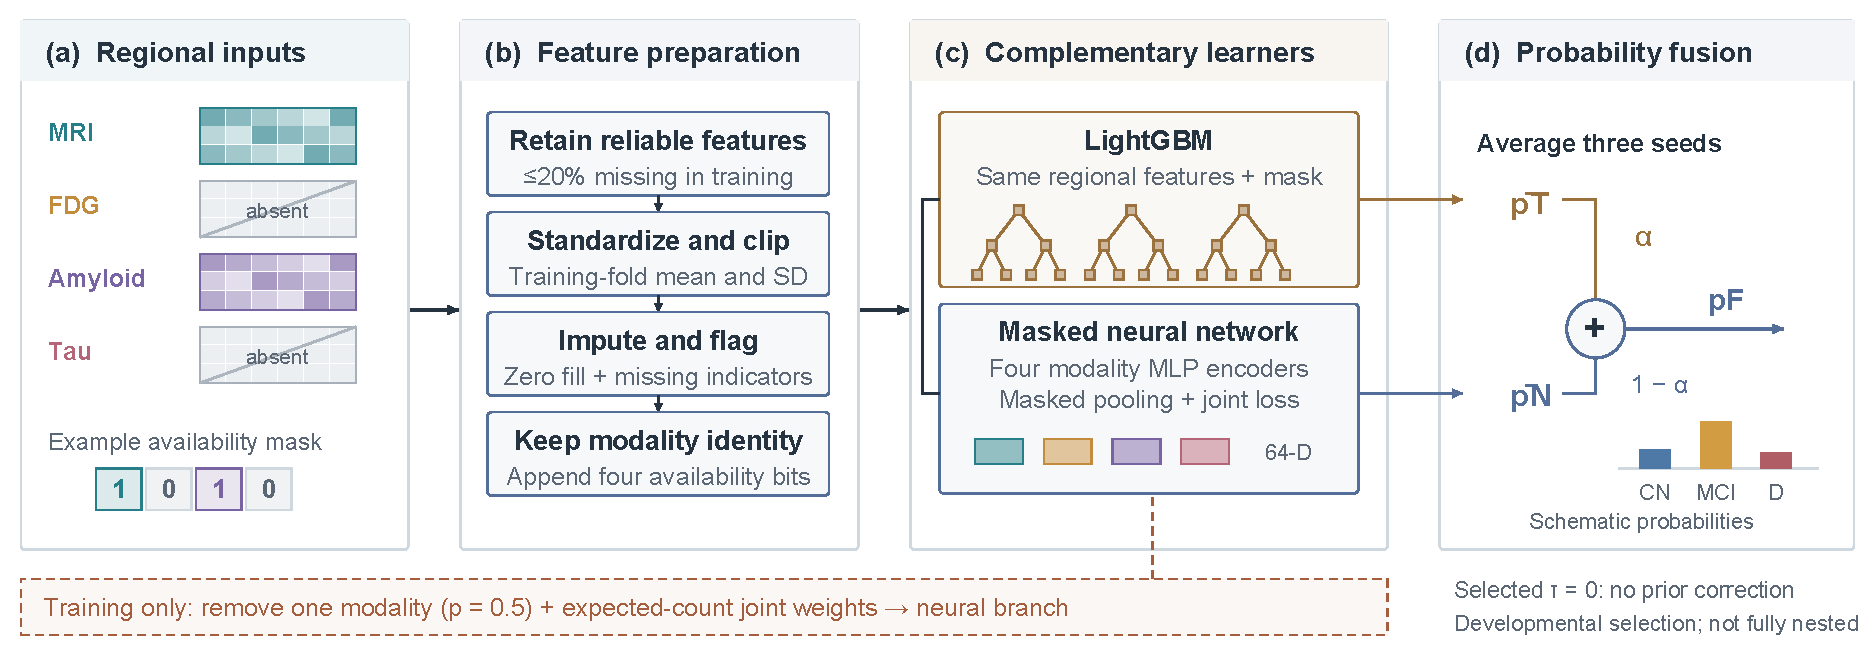
\includegraphics[width=\linewidth]{roi_pipeline}
\caption{AVF overview: regional inputs, training-fold preparation, complementary learners and probability fusion. Dashed links denote neural training controls. Tiles and output bars are schematic. Selection is developmental, not fully nested.}\label{fig:pipeline}
\end{figure}

\subsection{Complementary prediction branches}
\paragraph{Tree branch.} LightGBM receives concatenated regional blocks, feature-missing flags and four availability bits. It is trained without the neural cell-weighting objective. The reference and the fusion use the mean probabilities of the same three tree training seeds.

\paragraph{Neural branch.} Each modality has an MLP encoder producing $h_k\in\mathbb{R}^{64}$. It comprises linear, GELU and LayerNorm transformations with hidden dropout 0.1. A learned scalar gate $g$ defines masked pooling:
\begin{equation}
a_k=\frac{m_k\exp(g(h_k))}{\sum_j m_j\exp(g(h_j))},\qquad
h=\sum_k a_kh_k,\qquad z=f_{\theta}([h;m]).
\end{equation}
The implementation assigns absent gate scores $-10^9$ before softmax. The head maps the 68-value concatenation of the pooled token and mask to three logits. Softmax produces diagnosis probabilities. Figure~\ref{fig:architecture} expands feature preparation, modality encoders and masked pooling. The mask is a predictive input, so attention pooling should not be interpreted as eliminating missingness shortcuts.
\begin{figure}[pos=!ht]
\centering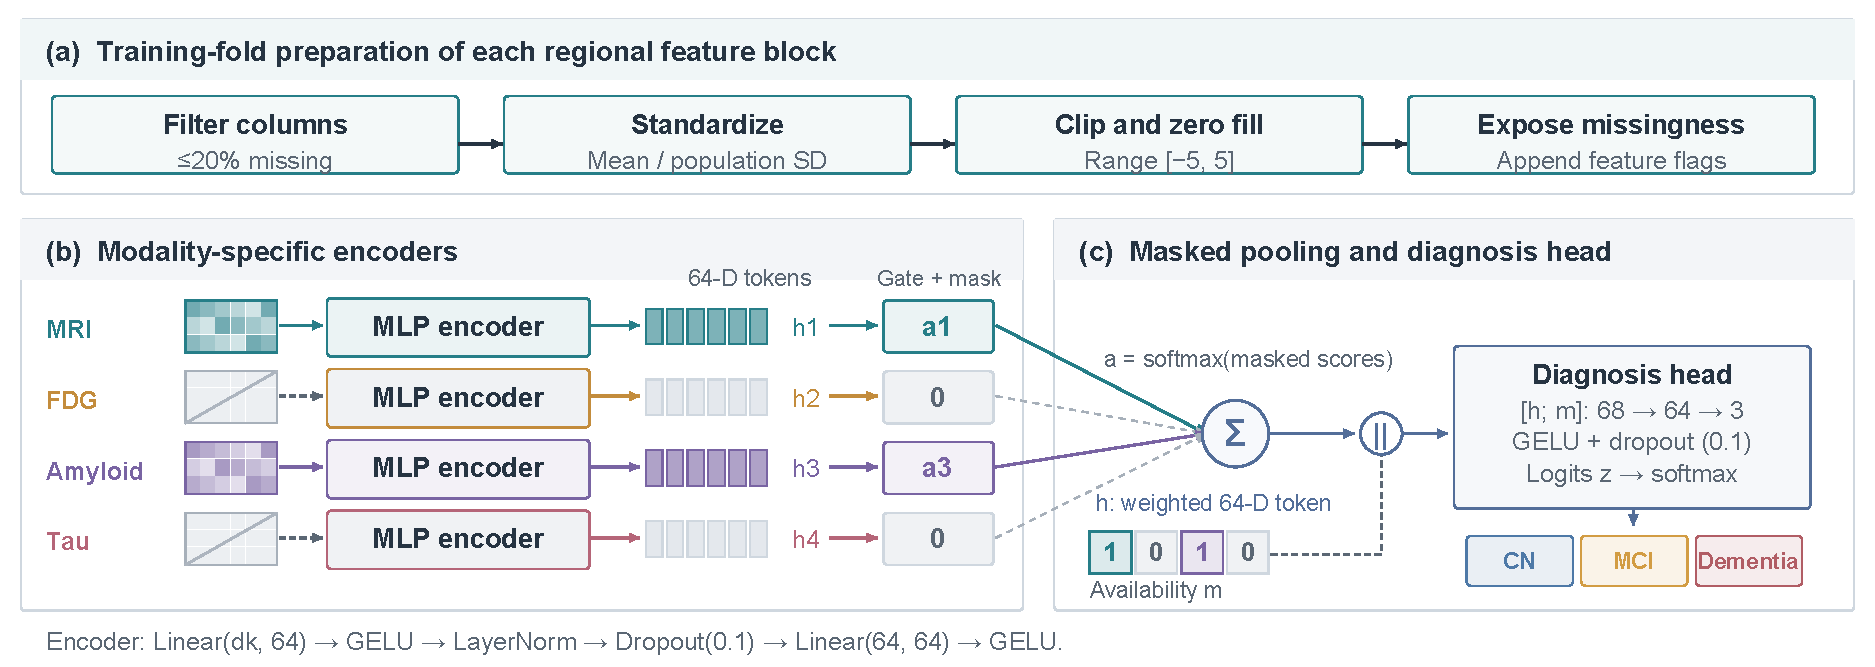
\includegraphics[width=\linewidth]{roi_architecture}
\caption{Neural branch: (a) feature preparation, (b) modality MLPs and 64-dimensional tokens, (c) masked pooling and diagnosis head. Grey tokens are excluded from pooling; encoder outputs need not be zero. The mask is illustrative.}\label{fig:architecture}
\end{figure}

\subsection{Modality dropout and joint weighting}
For episodes with at least two available modalities, training removes one uniformly chosen modality with probability 0.5 and updates its mask. Singleton episodes retain their modality. If $D(p)$ is the set of one-modality descendants of $p$ and $k(p)$ its number of modalities, expected effective counts are
\begin{equation}
E_{q,c}=\sum_p n_{p,c}T(q\mid p),\quad
T(q\mid p)=\begin{cases}
1 & k(p)=1,\ q=p,\\
1/2 & k(p)>1,\ q=p,\\
1/(2k(p)) & k(p)>1,\ q\in D(p),\\
0 & \text{otherwise}.
\end{cases}
\end{equation}
Thus 100 examples with MRI and FDG contribute expected masses 50 to the original pattern and 25 to each singleton descendant. Figure~\ref{fig:weighting} relates observed imbalance to this redistribution.
\begin{equation}
\widetilde w_{q,c}=\operatorname{clip}\!\left(\sqrt{\frac{N}{45(E_{q,c}+5)}},0.25,4\right),\qquad
w_{q,c}=\frac{\widetilde w_{q,c}}{N^{-1}\sum_{r,d}E_{r,d}\widetilde w_{r,d}}.
\end{equation}
The additive five smooths sparse counts; clipping occurs before mean-one normalization. Consequently, the final weights need not remain within the clipping bounds. The neural objective averages $w_{q_i,c_i}\operatorname{CE}(z_i,c_i)$ over a batch. No-dropout joint weighting substitutes natural counts for $E$. Class weighting uses an analogous three-class formula. These rules change influence rather than generating independent subjects.
\begin{figure}[pos=!ht]
\centering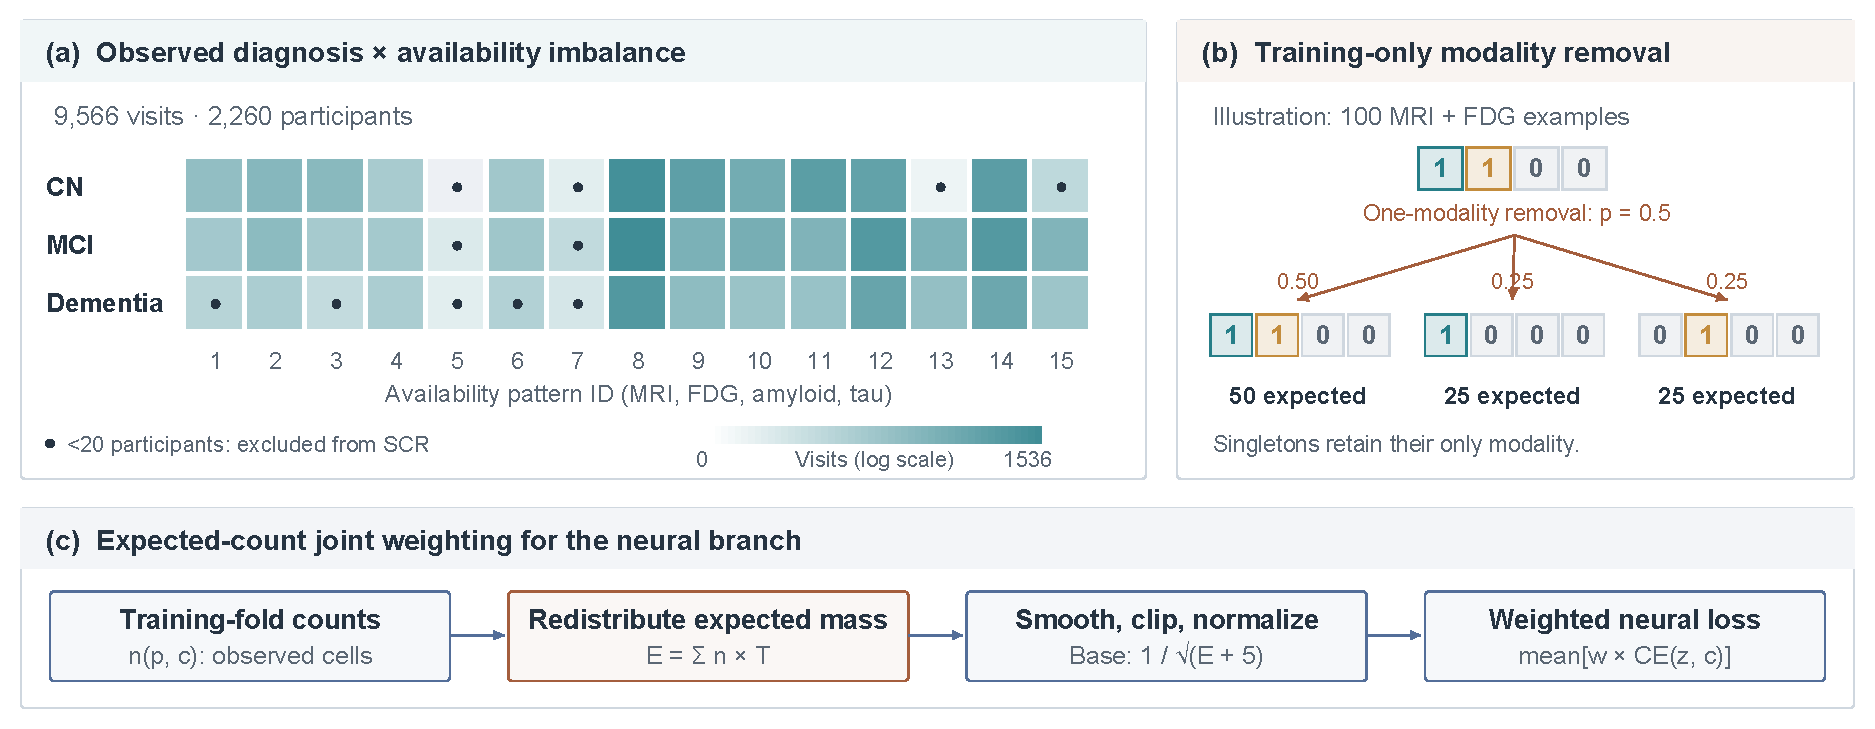
\includegraphics[width=\linewidth]{roi_joint_weighting}
\caption{Joint imbalance: (a) descriptive cohort counts; dots mark unsupported SCR cells, (b) illustrative dropout redistribution, (c) weighting from training-fold expected counts. Full-cohort counts are descriptive only.}\label{fig:weighting}
\end{figure}

\subsection{Probability fusion and its selection}
Let $\bar p^{T}$ and $\bar p^{N}$ denote probabilities averaged over three seeds for the tree and neural branches. AVF forms
\begin{equation}
p^{F}=\alpha\bar p^{T}+(1-\alpha)\bar p^{N}.
\end{equation}
For $\tau>0$, the archived search also allowed an optional prior correction,
\begin{equation}
p^{A}=\operatorname{softmax}\{\log\operatorname{clip}(p^{F},10^{-12},1)
+\tau[\log(1/3)-\log\operatorname{clip}(\bar P(c\mid p),10^{-6},1)]\},
\end{equation}
where $\bar P(c\mid p)=(n_{p,c}+20P(c))/(n_p+20)$ and $P(c)$ is the training-fold class frequency. Tuning averages the prior matrices of the other folds; application uses the target fold's training prior. At $\tau=0$, the implementation returns $p^F$ directly. The grid used $\alpha=0,0.05,\ldots,1$ and $\tau\in\{0,0.25,0.5,0.75,1,1.5\}$. It maximized natural macro-F1 on predictions from the other two folds, then applied the choice to the target fold. Selected tree weights were 0.55, 0.60 and 0.55; every selected $\tau$ was zero. The reported AVF is therefore the probability mixture without an active prior correction.

The leave-one-fold-out fusion search is not fully nested: the models that generate its tuning-fold predictions were trained on subjects from the target fold. Each reported validation fold also selected its own checkpoint epoch. A base learner does not fit its own held-out subjects, but that separation does not remove the selection dependencies. Generalization claims must therefore remain limited.

\section{Experimental design}\label{sec:setup}
\subsection{Shared folds and optimization}
Three StratifiedGroupKFold partitions (split seed 624) keep every participant's visits in the same fold. The held-out folds contain 3,190, 3,173 and 3,203 episodes from 761, 752 and 747 participants. Training seeds are 42, 1042 and 2042. Each training fold has its own fitted preprocessing. For each episode, we average probabilities across seeds before pooling predictions across folds and computing metrics. F1 is therefore computed from pooled predictions, not averaged across folds or seeds.

LightGBM uses learning rate 0.03, 31 leaves, minimum leaf size 20, feature and bagging fractions 0.8, up to 800 rounds and early stopping after 60 rounds using validation multiclass log loss. Regional networks use AdamW with learning rate $10^{-3}$, weight decay $10^{-2}$, batch size 128, at most 30 epochs, patience eight and gradient norm clipping at one. The best epoch maximizes natural validation macro-AUROC. Neural optimization uses CUDA; trees are CPU fitted. The original outer validation and test episodes are not inferred in this development revision.

\subsection{Factorial controls and comparator adaptations}
The factorial crosses weighting (none, class, joint) with modality dropout (off, on), yielding six arms. A seventh arm combines dropout with training-time logit adjustment: logits receive $\log[(E_{p,c}+5)/(\sum_d E_{p,d}+15)]$, with no additional sample weights and no offset at inference. Its fixed strength is one. This control is distinct from the optional post-hoc fusion correction.

TIMM-, Flex-MoE- and UniMIX-inspired regional adaptations share a 64-dimensional backbone and eight-expert, top-two routing configurations where applicable. They are trained under the local regional-input budget with their implemented auxiliary objectives. The Flex-style expert bank and curriculum differ from the published method, and the local UniMIX-style graph penalty does not reproduce the original graph-contrastive procedure. These are mechanism comparisons, not official reproductions or comparisons with published headline scores.

\subsection{Metrics and uncertainty}
Macro-AUROC averages three one-versus-rest AUROCs. Macro-F1 averages per-class F1; balanced accuracy averages class recall. Supported-cell recall (SCR) is
\begin{equation}
\operatorname{SCR}=\frac{1}{|\mathcal S|}\sum_{(p,c)\in\mathcal S}
\frac{\sum_i\mathbb 1[p_i=p,c_i=c,\hat c_i=c]}{\sum_i\mathbb 1[p_i=p,c_i=c]}.
\end{equation}
The fixed natural support set $\mathcal S$ contains 34 cells with at least 20 distinct participants. Support is participant-based, but recall within a cell is visit-weighted. SCR is not a worst-cell guarantee and does not cover all sparse cells.

The paired bootstrap samples participants with replacement and retains all their visits. Each resample uses the same participants for every method. We retain the archived 1,000-resample percentile intervals for the primary natural comparison. These intervals condition on the fitted and selected models; training is not rerun, and exploration across the family of models is not accounted for. Point differences are recomputed on the original pooled predictions and can differ slightly from archived bootstrap mean differences.

\subsection{Stress-test restriction and artifact replay}
Archived experiments include a synthetic drop-one condition, but the replay audit found different effective masks in the factorial and comparator families. Part of the random selection did not use the supplied generator. Those archived predictions cannot support cross-family stress superiority claims. Correctly paired masks require a controlled rerun; relabelling existing predictions would not repair the mismatch. All primary results reported here use natural availability.

The revision reconstructs all natural table rows from archived probabilities without importing training modules or running new inference. It checks episode and label alignment, normalized probabilities, saved subject partitions, fixed cell support and the AVF mixture. It preserves the original experiment records; provenance checks do not establish independent test validity.

\section{Results}\label{sec:results}
\subsection{Primary natural-availability comparison}
Table~\ref{tab:natural} reports replayed natural metrics on the same 9,566 episodes with a fixed support set. AVF attains AUROC 0.7969, macro-F1 0.6194, balanced accuracy 0.6251 and SCR 0.6043. The seed-ensembled LightGBM reference scores 0.7937, 0.6014, 0.5952 and 0.5685. Figure~\ref{fig:performance} highlights the class- and cell-sensitive comparison.
\begin{table}[pos=!ht]
\caption{ROI-only natural evaluation. Values are pooled metrics after averaging three seeds' probabilities per episode. All rows use the same 34 supported cells for SCR. Comparator rows are local adaptations.}\label{tab:natural}
\begin{tabular*}{\tblwidth}{@{} LCCCC @{}}\toprule
Method & AUROC & Macro F1 & BAcc & SCR \\ \midrule
Plain neural & 0.781 & 0.598 & 0.598 & 0.543 \\
+ class weights (CW) & 0.781 & 0.597 & 0.619 & 0.564 \\
+ joint weights (JW) & 0.776 & 0.591 & 0.615 & 0.583 \\
+ modality dropout (MD) & 0.782 & 0.600 & 0.599 & 0.547 \\
+ CW + MD & 0.784 & 0.601 & 0.621 & 0.573 \\
+ JW + MD & 0.778 & 0.593 & 0.621 & 0.585 \\
+ logit adjustment + MD & 0.769 & 0.579 & 0.617 & 0.584 \\
LightGBM seed ensemble & 0.794 & 0.601 & 0.595 & 0.568 \\
TIMM-inspired adaptation & 0.785 & 0.603 & 0.605 & 0.567 \\
Flex-MoE-inspired adaptation & 0.789 & 0.607 & 0.610 & 0.564 \\
UniMIX-inspired adaptation & 0.793 & 0.608 & 0.615 & 0.581 \\
\textbf{AVF (proposed)} & 0.797 & 0.619 & 0.625 & 0.604 \\
\bottomrule\end{tabular*}
\end{table}
\begin{figure}[pos=!ht]
\centering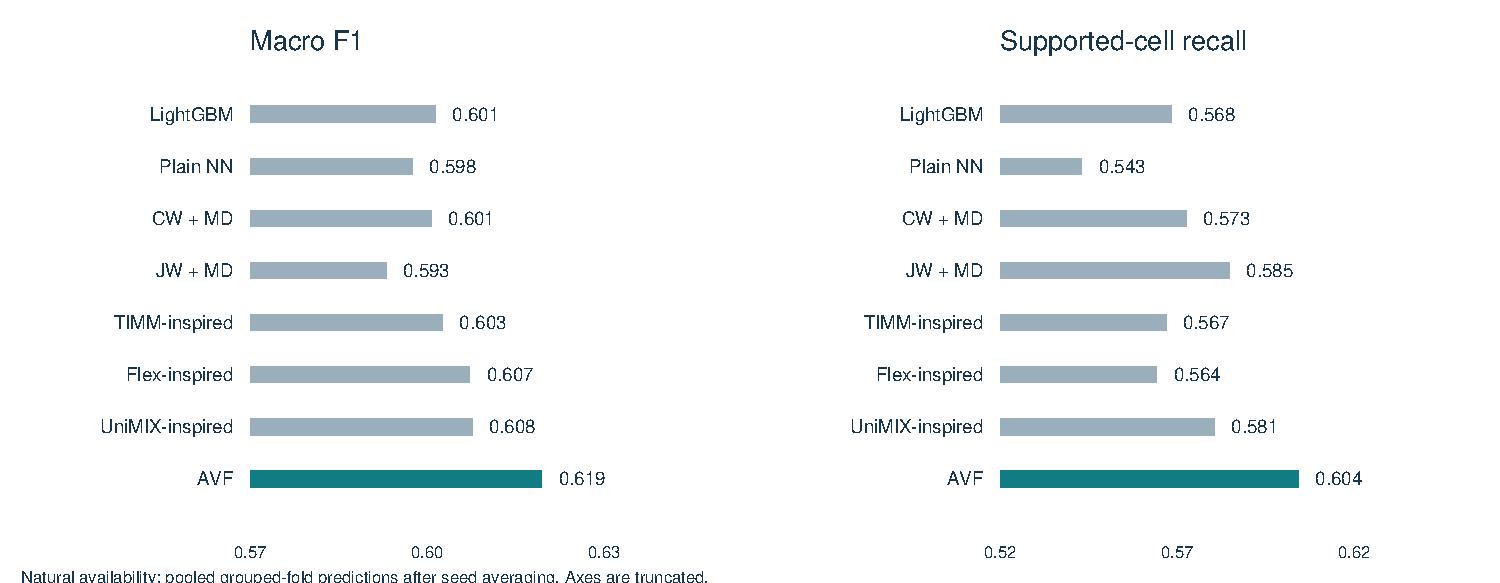
\includegraphics[width=\linewidth]{roi_performance}
\caption{Natural macro-F1 and SCR. The tree is a strong reference; joint balancing alone improves cell recall but does not dominate every metric. Axes are truncated to show differences and the figure does not display uncertainty.}\label{fig:performance}
\end{figure}

Table~\ref{tab:uncertainty} reports the original-sample differences alongside bootstrap intervals. The paired participant intervals support F1 and SCR gains for AVF, whereas the AUROC interval crosses zero. These intervals remain exploratory: they condition on the selected models and do not account for all selection or multiplicity.
\begin{table}[pos=!ht]
\caption{AVF minus seed-ensembled LightGBM. Point differences are replayed; 95\% percentile intervals are retained from the archived 1,000-resample participant bootstrap.}\label{tab:uncertainty}
\begin{tabular*}{\tblwidth}{@{} LCC @{}}\toprule
Metric & Point difference & 95\% interval \\ \midrule
Macro-AUROC & +0.00318 & [$-0.000052$, +0.00610] \\
Macro-F1 & +0.01803 & [+0.01021, +0.02559] \\
SCR & +0.03577 & [+0.02027, +0.05145] \\
Balanced accuracy & +0.02986 & Not estimated in this archived contrast \\
\bottomrule\end{tabular*}
\end{table}

\subsection{Factorial evidence and local comparator mechanisms}
Relative to the plain neural model, joint weighting with dropout raises SCR from 0.5431 to 0.5848 and balanced accuracy from 0.5984 to 0.6208, while AUROC falls from 0.7807 to 0.7783. Class weighting plus dropout instead yields macro-F1 0.6007 and SCR 0.5726. Thus joint weighting trades some discrimination and F1 for cell coverage; it is not a uniformly better loss. Fixed training-time logit adjustment gives the lowest AUROC and F1 among these arms, despite higher cell recall than the plain reference.

The three local comparator adaptations reach macro-F1 0.6027--0.6076. AVF has higher pooled natural F1 and SCR point estimates than all three. This ranking applies to the adaptations under the shared regional inputs and local training budget; it does not establish superiority over the published original systems.

\subsection{Member ablation and per-cell changes}
The archived member ablation in Table~\ref{tab:member} shows that fusion with a plain neural model already raises F1 to 0.6089 from the tree's 0.6014. Part of the gain thus comes from generic ensembling. Joint-plus-dropout fusion has the highest SCR and balanced accuracy among the tested members, while class-plus-dropout fusion has slightly higher AUROC and F1. AVF represents a cell-sensitive tradeoff, not a configuration that wins every metric. The ablation does not independently isolate any component's causal contribution.
\begin{table}[pos=!ht]
\caption{Tree fusion with alternative neural members. Archived rounded member-ablation values are shown to four decimals. Codes correspond to the factorial arms in Table~\ref{tab:natural}.}\label{tab:member}
\begin{tabular*}{\tblwidth}{@{} LCCCC @{}}\toprule
Neural member & AUROC & Macro F1 & BAcc & SCR \\ \midrule
none\_no\_drop & 0.7954 & 0.6089 & 0.6063 & 0.5699 \\
class\_no\_drop & 0.7970 & 0.6162 & 0.6181 & 0.5837 \\
joint\_no\_drop & 0.7964 & 0.6168 & 0.6204 & 0.5923 \\
none\_drop & 0.7968 & 0.6127 & 0.6087 & 0.5760 \\
class\_drop & 0.7977 & 0.6202 & 0.6235 & 0.5921 \\
joint\_drop & 0.7969 & 0.6194 & 0.6251 & 0.6043 \\
logitadj\_drop & 0.7964 & 0.6158 & 0.6220 & 0.5974 \\
\bottomrule\end{tabular*}
\end{table}
Across the 34 supported natural cells, 19 improve relative to LightGBM and the mean recall change is +0.03577 (Figure~\ref{fig:cells}). Several cells worsen, including common MCI patterns. The mean gain therefore does not establish improvement in every cell or in the worst cell. Sparse unsupported cells are outside the SCR estimate.
\begin{figure}[pos=!ht]
\centering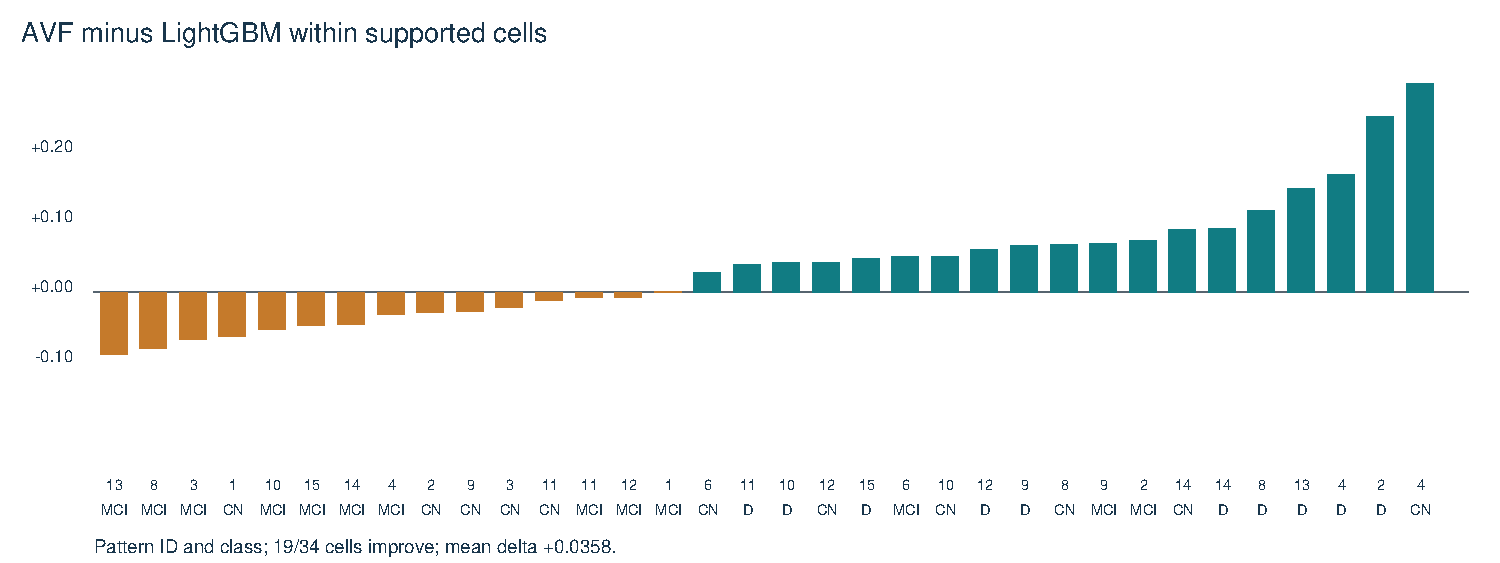
\includegraphics[width=\linewidth]{roi_cell_deltas}
\caption{AVF minus LightGBM recall in each supported class--pattern cell, ordered by difference. Pattern IDs use the four-bit encoding; D denotes dementia. Both improvements and regressions are retained.}\label{fig:cells}
\end{figure}

\section{Discussion}
\subsection{What the results support}
AVF improves macro-F1 and supported-cell recall in this development evaluation. Joint weighting raises cell recall relative to the plain neural reference but reduces AUROC. Fusion retains strong ranking performance and improves class-level decisions, although its natural AUROC advantage over seed-ensembled LightGBM remains uncertain. The evidence does not support a uniformly superior classifier.

Generic ensembling improves some metrics. The joint-weighted member has the highest SCR among seven tested members, whereas class-weighted fusion yields slightly higher macro-F1 and AUROC. The results are consistent with complementary errors but do not attribute the entire gain causally to joint weighting. Deployment would require a prespecified metric and independent validation of calibration and error costs.

Regional summaries permit studying imbalance without learning voxel representations. The evidence does not establish image-level representation quality, improved raw-image diagnosis or superiority over the original published multimodal systems. Availability awareness here means explicit model inputs and a training design, not immunity to acquisition-policy shortcuts.

\subsection{Limitations and the next validation step}
The main limitation is model selection within a development evaluation. Checkpoint selection reuses the reported fold, and fusion selection is not fully nested because tuning-fold learners saw target-fold subjects during fitting. Repeated method exploration can further favour the observed configuration \citep{cawley2010selection}. Participant bootstrap intervals quantify conditional sample uncertainty without removing these dependencies. The next evaluation must lock the scope, metric, weighting rule and fusion-selection procedure. All selection must occur within each outer training set, followed by a single evaluation on an untouched outer or external cohort.

Repeated visits increase the number of observations without adding independent participants. SCR excludes cells below the support threshold and weights visits within each retained cell. Larger or more diverse tau and rare-pattern samples could change the conclusions. The analysis also inherits alignment tolerances, regional processing differences and diagnosis uncertainty. It establishes no prospective clinical validity, causal explanation, demographic fairness guarantee or worst-cell guarantee.

The comparator mechanisms are simplified local adaptations, and faithful original implementations or a different training budget may change their rankings. The stress-mask mismatch also prevents interpreting archived cross-family drop-one intervals as robustness evidence. These limitations qualify the reported comparisons; unfavourable controls remain part of the analysis.

\section{Conclusion}
On this participant-grouped ADNI regional-feature development cohort, AVF reaches macro-F1 0.619 and SCR 0.604 versus 0.601 and 0.568 for seed-ensembled LightGBM. Joint balancing changes the ranking--recall tradeoff but is not universally optimal. AUROC gains remain small and uncertain. Strong generalization claims require locked nested or external evaluation.

\paragraph{Data and code availability.} Code, manuscript sources, vector figures and aggregate results are available at \url{https://github.com/DevanshSurana7214/AVF}. ADNI participant data require authorized access and are not redistributed. The repository distinguishes extracted historical components from release utilities and documents the private inputs required for a complete study replay.

\paragraph{Declaration of generative AI assistance.} Generative AI assisted implementation, analysis and manuscript drafting. The authors are responsible for verifying the code, results, citations and final claims. Contribution statements and any institutional disclosure requirements must reflect the authors' actual work.

\printcredits
\bibliographystyle{elsarticle-num-names}
\bibliography{references}
\end{document}
